\documentclass[twoside]{article}


% ------
% Fonts and typesetting settings
\usepackage[sc]{mathpazo}
\usepackage[T1]{fontenc}
\linespread{1.05} % Palatino needs more space between lines
\usepackage{microtype}
\usepackage{amsmath}
\usepackage{color}
\usepackage{float}
% ------
% Page layout
\usepackage[hmarginratio=1:1,top=32mm,columnsep=20pt]{geometry}
\usepackage[font=it]{caption}
\usepackage{paralist}
\usepackage{multicol}

% ------
% Lettrines
\usepackage{lettrine}


% ------
% Abstract
\usepackage{abstract}
	\renewcommand{\abstractnamefont}{\normalfont\bfseries}
	\renewcommand{\abstracttextfont}{\normalfont\small\itshape}


% ------
% Titling (section/subsection)
\usepackage{titlesec}
\renewcommand\thesection{\Roman{section}}
\titleformat{\section}[block]{\large\scshape\centering}{\thesection.}{1em}{}


% ------
% Header/footer
\usepackage{fancyhdr}
	\pagestyle{fancy}
	\fancyhead{}
	\fancyfoot{}
	\fancyhead[C]{Journal paper template $\bullet$ April 2012 $\bullet$ Vol. XXI, No. 1}
	\fancyfoot[RO,LE]{\thepage}

\usepackage{graphicx}
\graphicspath{{./Figures/}}
\usepackage{caption}
% ------
% Clickable URLs (optional)
\usepackage{hyperref}

% ------
% Maketitle metadata
\title{\vspace{-15mm}%
	\fontsize{24pt}{10pt}\selectfont
	\textbf{An experimental comparison of several classification algorithms based mouse gesture recognition }
	}	
\author{%
	\large
	\textsc{Salwa O. Slim} \\[2mm]
	\normalsize	Computer Science Department,
	\\Faculty of Computers and Information, Helwan University.
	\vspace{-5mm}
	}
\date{}



%%%%%%%%%%%%%%%%%%%%%%%%
\begin{document}

\maketitle
\thispagestyle{fancy}

\begin{abstract}
\noindent The simply identified the mouse gestures: The user gestures a shape while holding a mouse button and if the shape is identified by using recognition algorithm, the appropriate action is executed. Mouse gestures can be used in a different application like Hindi digits recognition, Arabic-Urdu alphabet script recognition in real-time and in the login security system. Developing technique to recognize mouse gestures with high quality is challenging. This paper presents a performance analysis and comparison of six classifier algorithms used in mouse gesture recognition. We studied and compared the classification algorithms, which are K-nearest Neighbor, Artificial Neural Network, Na\"{i}ve Bayes, Dynamic Time Warping, \$1 recognizer and Support Vector Machine . The comparison applied on two different data sets (Hindi digits and Unistroke shapes datasets).\\[2mm]
\noindent Keywords - mouse recognition, K-nearest Neighbor, Artificial Neural Network, Na\"{i}ve Bayes, Dynamic Time Warping, \$1 recognizer, Support Vector Machine 
\end{abstract}
	

\begin{multicols}{2}
\section{Introduction}
\paragraph{}The traditional modulations of the human computer interaction are keyboard and mouse. However, there are some of new modulates in the style of interaction based on the standard channels such as a type of gesture performed with the mouse. Some of the requirements are needed to increase the level of login security. It can be achieved by integrating existing systems (the traditional way of accepting password through the keyboard) with a user signature which can be identified using mouse gesture recognition [1] and biometric authentication for web system [2]. The mouse gesture can be used to recognize the Hindi digits [3] and Arabic-Urdu alphabet script in real-time using artificial neural network [4]. There are some desktop applications support mouse gestures. The Opera Web Browser, for example, uses mouse gestures to navigate and manage windows.
The mouse gesture continues and directed sequence of moues cursor movement with distinguished the start and the end of movement. the directions are very important to recognize the gestures movement (right, left, top, down). The gesture may be use the combination of mouse or keyboard keys. In this paper, gestures are marked by pressing the right button. There are two phases in the mouse gesture recognition a pre-processing phase(Resample) that reduces the number of the points of mouse gesture path and classification phase that uses classifier algorithm to categorize the gesture. 
The purpose of this paper presents the comparative study of six classifier algorithms applied to uni-strock mouse gesture dataset: Artificial Neural Network (ANN), K-Nearest Neighbor (KNN), Na\"{i}ve Bayes (NB), \$1 Recognize, Dynamic Time Warping (DTW), and Support Vector Machines(SVM). We analyze and present the accuracy of each algorithm and change the size of data training to compare the algorithms to know the best algorithm with high accuracy when the training data are few. The rest of the paper is as follows, First we review related work in section2. Section3 explains the classification methods. The experimental methodology and results are explained in section4. Section5 discusses the values obtained and Conclusion. 

\section{Related Work}
There are many comparative studies on classification algorithms in different applications [12] and datasets like the study of  Na\"{i}ve Bayes (NB) and HMM on hand gesture [5], the paper [6] applied  two different hand datasets to compare classification algorithms (k-Nearest Neighbor,  Na\"{i}ve Bayes, Artificial Neural Network, Support Vector Machines), and the comparative classification algorithms in data mining [9]. Several algorithms are used for skin color pixel classification like piecewise linear classifiers, the Bayesian classifier, Gaussian classifiers and the multilayer perception [7]. We can compare the effectiveness of various feature selection methods by applying classification algorithms (k-NN, C4.5, NB, and SVM) [8]. The authors [10] compares three classification algorithms on five real datasets. weka tool is used to apply different classification algorithms (Na\"{i}ve Bayes classifier, SVM classifier, KNN classifier and C4.5 Decision Tree Classifier) on the animal dataset [11]. Machine learning algorithms can be used in many fields like, classifying human physical activity from on-body accelerometers [18] [13] and mobile phone [14], automatic road-sign detection [19] [20], face recognition [15],  classification of robotic soccer formations [17], and automatic recognition of a musical gesture by a computer [16].
Machine learning algorithms can be used in many fields like, classifying human physical activity from on-body accelerometers [18] automatic road-sign detection [19, 20] , ace recognition [15],  classification of robotic soccer formations [17], and automatic recognition of a musical gesture by a computer [16].

\section{Classification Methods}

\subsection*{Na\"{i}ve Bayes Classification}
It is the simple statistical Bayesian Classifier[21]. It assumes the features are conditionally independent[22]. There are k classes $C_{1}, C_{2} \cdots C_{k}$  With features X=$X_{1}, X_{2} \cdots X_{n}$ ,The Classification of such classes is derived using the maximum posterior P($C_{i}$|X). This can be derived from Bayes' theorem.

\begin{equation}
\label{Bayes' theorem}
P(C_{k}|X)=\frac{P(C_{k})P(X|C_{k})}{P(X))}
\end{equation}
\\OR\\
\begin{equation}
\label{Bayes' theorem1}
Posterior=\frac{prior\items likelihood}{evidence}
\end{equation}
Where
\begin{itemize}
\item P($C_K$|X) is posterior ( the probability of the class $C_k$ . being X feature)
\item P($C_K$) is prior (the probability of the class $C_k$).
\item P(X|$C_K$) is Likelihood(the probability of X feature belong to the Class $C_k$.
\item P(X) is evidence( describe by measure the probability of features).
\end{itemize}

\subsection*{K-Nearest Neighbor Classification}
K‐NN is a supervised learning algorithm, where the user partitions the given dataset into a number of clusters. There are two phases-Training and testing phase- in the algorithm.The Training phase stores the features and the class label of the training sets. New data are classified based on the voting criteria [23].  It measures the maximum likelihood estimation of the class. The algorithm assigns the object to the most frequently labeled class by using Euclidean distance measurement. Distances are calculated from all training objects to test object using the appropriate K value [24]. the changing in K can be changes the accuracy of the algorithm but in this paper the k=1

\subsection*{Neural Network}
The multilayer perception (MLP) is a feed-forward neural network [25] that has been used extensively in classification and regression. The neural network consists of an input layer, one or more hidden layers, and output layer. Each layer consists of one or more neurons, which directly linked with neurons from the previous and the next layer. Each neural network has several inputs and several outputs. The neural takes the output values from several neurons in the previous layer as input and then passes the response to several neurons in the next layer. The values retrieved from the previous layer are summed up with certain weights, individual for each neuron, plus the bias term. The sum is transformed using the activation function that may be different for different neurons. 

\subsection*{Support Vector Machine}
SVM is based on statistical learning theory. The goal of the classifier is determining the location of decision boundaries also known as Hyperplane [26]. Hyperplane separates objects of different classes by drawing separating lines among the objects. SVM classifies the data by creating Hyperplanes in a multidimensional space. In the training phase of SVM finds a unique global minimum.

\subsection*{Dynamic Time warping}
DTW is effective for time series classification because of its non-linear mapping capability. It finds an optimal match between two sequences by allowing a non-linear mapping of one sequence to another, and minimizing the distance between two sequences.
Suppose we have two time series X and Y, of length n and m respectively, where:$ X= x_1 ,x_2 ,\cdots,x_i ,\cdots,x_n$  and  y = $y_1 ,y_2 ,\cdots,y_j ,\cdots,y_m $To align two sequences using DTW we construct an n-by-m matrix where the ($i^{th} , j^{th} $) element of the matrix contains the distance d($x_i$ ,$y_j$) between the two points $x_i $ and$y_j $ (With Euclidean distance, d($x_i ,y_j ) = (x_i - y_j )^ 2 )$. Each matrix element (i,j) corresponds to the alignment between the points$ x_i $ and$ y_j$, you can show warping path in Fig \ref{fig:DTWGraph}.

%\begin{figure*}[h]
	%
		%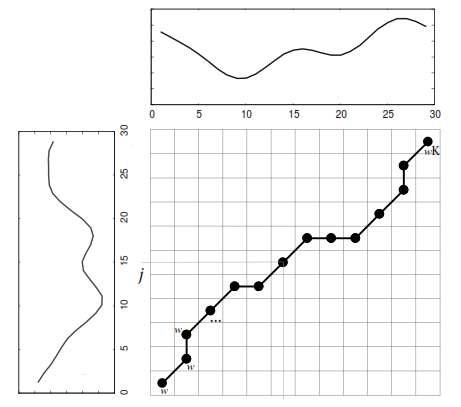
\includegraphics[natwidth=100, natheight=200,width=0.05\textwidth]{../Figures/DTWGraph.png}
	%\caption{Dynamic Time Warping matrix}
	%\label{fig:DTWGraph}
%\end{figure*}

	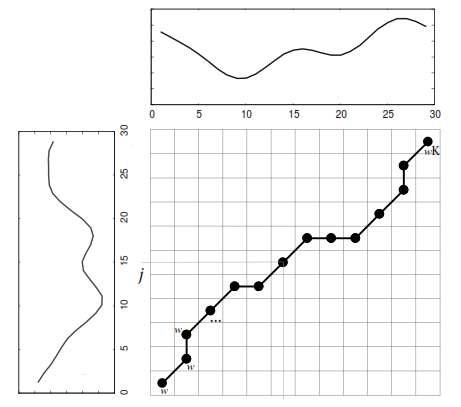
\includegraphics[scale=0.5]{../Figures/DTWGraph.png}
	\captionof{figure}{Dynamic Time Warping}
	\label{fig:DTWGraph}


A warping path W, is a contiguous set of matrix elements that defines a mapping between x and y. The $k^{th}$ element of W is defined as$w_k = (i,j)_k $ so we have:
\begin{multline}
$W= w_1, w_2, \dotc ,w_k$ \\ max(m,n) \leq K < m+n-1 
\end{multline}
The warping path has several constraints[27].
\begin{itemize}
\item Boundary conditions: the starting and ending points of warping path have to be the first and the last points of the path matrix.
\item Continuity: the path can advance one step at a time.
\item Monotonicity: the points in W have to be monotonically spaced in time. the experimental section display the comparison between resample and non-resample the points of the path. 
\end{itemize}

\subsection*{\$1 Gesture Recognition}
The \$1 Unistroke Recognizer is designed for rapid prototyping of gesture-based user interfaces. \$1 is an instance-based nearest neighbor classifier with a Euclidean Distance measurement.
The gesture of user display in a set of candidate points C, and we must determine which set of previously recorded template points Ti it most closely matches. Candidate and template points are usually obtained through interactive means by some path-making instrument moving through a position-sensing region. 

\section {Experimental methodology and Results}
The dataset with different set of mouse gesture have been used to test the classification algorithms.
The second dataset are from the website for \$1 [30] and contains 16 gestures that are illustrated in Fig \ref{fig:unistrokes}. The gestures are collected by Pocket PC recorder in the form xml file.

	
	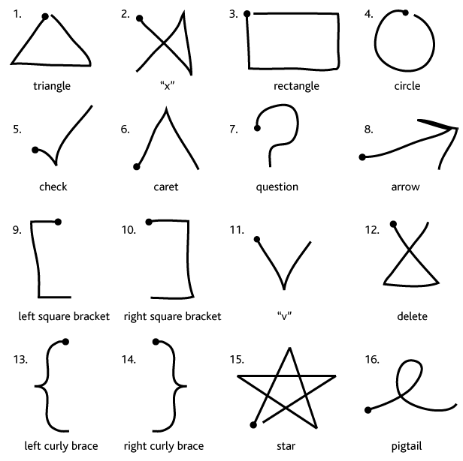
\includegraphics[scale=0.5]{../Figures/unistrokes.png}
	\caption{Unistroke gestures}
	\label{fig:unistrokes}


The first step for organizing the data was converting the XML files to TXT files. We created application in C++ to apply two datasets on six classification algorithms for the comparison study.

The common step in all algorithms is the resample phase (resample the points of the gesture N) in order to unite the number of points in the training and testing gesture to easy compare between them except for Dynamic time warping (DTW) algorithm which used the original points without need to resample the gesture points. The settings and parameters of the classifiers is an important aspect to take into account. Thus, we set N=64 in the resample phase, k=1 in the K-NN algorithm.
Table\ref{tab:Table1} displays the accuracy and the execution time-with minutes-of the classifier algorithm. The accuracy is calculated by using 1 sample for each gesture in the training data and 30 samples for each gesture in the testing data.
\begin{table*}[t]
	\centering
		\begin{tabular}
			{||l|c|c|c|c|c|c|c|c|c|c|r|}\hline
		\multicolumn{2}{||l}{K-NN}& \multicolumn{2}{|c}{ANN} &\multicolumn{2}{|c}{Naive}&\multicolumn{2}{|c}{DTW}&\multicolumn{2}{|c}{1\$}& \multicolumn{2}{|r|}{SVM}\\ \hline
			\midrule
			Accuracy \%&T & \%&T & \%&T & \%&T & \%&T & \%&T \\ \hline
			62.5&0.00055	& 58.33&0.02 & 62.5&0.10 & 95&4.3 & 85&0.22 & 62.5&0.0002 \\ \hline
		\end{tabular}
	\caption{The Accuracy and Execution time using 1 sample for training}
	\label{tab:Table1}
\end{table*}
The size of the training data effect on the accuracy of the algorithm, Table\ref{tab:Table2} show the effectiveness of training data on the accuracy of the algorithm and time spent.
The data size for training and testing are 300, 30 samples for each gesture.
\begin{table*}[t]
	\centering
		\begin{tabular}
			{||l|c|c|c|c|c|c|c|c|c|c|r|}\hline
						\multicolumn{2}{||l}{K-NN}& \multicolumn{2}{|c}{ANN} &\multicolumn{2}{|c}{Naive}&\multicolumn{2}{|c}{DTW}&\multicolumn{2}{|c}{1\$}& \multicolumn{2}{|r|}{SVM}\\ \hline
			\midrule
			Accuracy \%&T & \%&T & \%&T & \%&T & \%&T & \%&T \\ \hline
			98.75&0.012	& 91.66&4.29 & 99.1&0.18 & 100&35420 & 100&101.9 & 99.6&0.08 \\ \hline
		\end{tabular}
	\caption{The Accuracy and Execution time using 300 samples for training}
	\label{tab:Table2}
\end{table*}
DTW algorithm is the only one from six implemented algorithms which exist in this paper doesn't resample the gesture. The Figure\ref{fig:Resample-NonResample} compares the error rate between DTW algorithm results with resample the gesture (N=64) and the results without resample (original points) the gesture.

	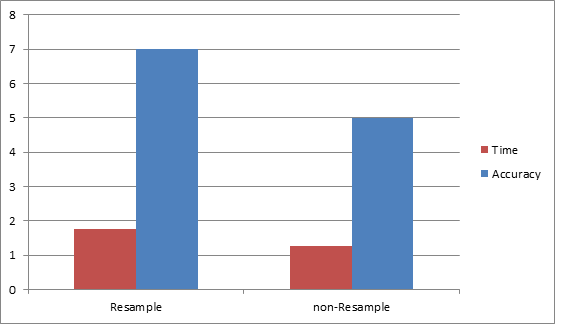
\includegraphics[scale=0.5]{../Figures/Resample-NonResample.png}
	\captionof{figure}{DTW error rate with resample and without resample phase}
	\label{fig:Resample-NonResample}

The Figure\ref{fig:DifferentNumpoint} displays the effective of DTW results when the number of points in the resample phase are changed. X-axis is the number of Resample points (N=10, 20, 30 \cdots 100).

		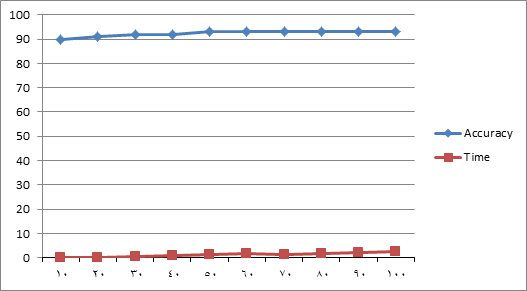
\includegraphics[scale=0.5]{../Figures/DifferentNumpoint.png}
	\caption{DTW with different number of resample points}
	\label{fig:DifferentNumpoint}

\section {Discussion and Conclusion}
\paragraph{}The size of training data effect on the accuracy of the algorithm. In the Table\ref{tab:Table1}, the classifiers are used small training data (one sample for each gesture) and the testing data is 30 samples for each gesture. The Accuracy of all classifiers is low, but the highest one is DTW Accuracy. DTW execution time is the highest. 1\$ accuracy is the best after DTW. The K-NN, SVM, Naïve are the same accuracy ,but the K-NN is the best because it takes less time.
When we increase the size of training data, the accuracy will also increase, as a display in the Table\ref{tab:Table2}. The accuracy of all classifiers increased. The training data samples are 300 samples for each gesture. The highest accuracy in the Table\ref{tab:Table2} are DTW and 1\$ Accuracy but the best one is 1\$ because it's time execution is less than DTW.
The DTW classifier doesn't include the resample phase. Does that phase may effect on the execution time or the accuracy of the classifier? the Fig \ref{fig:Resample-NonResample} will answer the previous question. In the Fig \ref{fig:Resample-NonResample}, the error rate of DTW with resample phase is higher than DTW without resample phase and the execution time of DTW with resample is higher than DTW without resample phase.
Fig \ref{fig:DifferentNumpoint} displays the effect of resample phase on accuracy and execution time. From the range 10 to 50 points, the accuracy is growing and from 60 to 100 the accuracy is the same approximately. The time is growing when the number of sample points is growing.
\paragraph{}The training size data effects on the accuracy and execution time of any classifier.  Dynamic Time Warping has the highest accuracy when the size of training data is small, but it takes more time. The accuracy of 1\$ is the same DTW when the size of data training is large and 1\$ execution time is less than DTW. DTW without resample phase is better than DTW with the resample phase.
\clearpage
\section{Refrences}
\end{multicols}

\end{document}
